\subsection{Gas ideali}
Un gas ideale è costituito da particelle puntiformi, che non abbiano un proprio volume, e contenute in un recipiente cui è praticato il vuoto in modo da avere solo poche particelle del gase e dove abbiamo dei misuratori di temperatura e pressione.

Definiamo un gase "ideale" quando esso si trova a bassa pressione, quindi rarefatto e ad alta temperatura.

In queste condizioni è ragionevole assumere che non esistano interazioni fra le varie particelle, per cui esse si muovono in modo del tutto casuale. Qualora dovessero esserci urti, si assumono essere perfettamente elastici.

Un gas occupa l'intero volume che trova a sua disposizione ed esercita una pressione dovuta agli urti delle particelle del gas sulle superfici interne del recipiente che lo contiene.

Le proprietà di un gas sono determinate dalla sua pressione a la sua temperatura.

\vspace{0.2cm}La pressione, cioè la forza esercitata sulle pareti, ha come unità di misura l'\textit{atmosfera (atm)}. Inoltre $1 \; atm=760 \; mmHg=1 \; Torr$. Nel S.I. l'unità di misura è il \textit{Pascal (Pa)}, per cui

$$P=N/m^2=\big[ (kg \cdot m)/s^2 \big]/m^2=(kg \cdot m)(s^2 \cdot m^2)$$
$$\rightarrow P=kg/(s^2 \cdot m)$$

Spesso nelle bombole l'unità di misura è il \textit{bar}. 1 bar equivale a $10^5 \; Pa$.

LA temperatura si misura in gradi centigradi (°C) o in gradi Kelvin (K).
\subsection{Significato molecolare della pressione}
La pressione è dovuta agli urti delle particelle contro le pareti del recipiente che lo contiene ed è la stessa in tutti i suoi punti.
\subsection{Significato molecolare della temperatura}
Supponiamo di avere un gas dentro un contenitore chiuso e di riscaldarlo mantenendo costante il suo volue. Ci accorgiamo che aumenta la pressione, cioè aumenta il numero di urti delle particelle nell'unità di tempo. Se aumentano gli urti, aumenterà la velocità delle particelle. Dalla teoria cinetica molecolare sappiamo che l'energia cinetica di una particella è pari a $E_k=3/2 K_bT$, dove $K_b$ è la costante di Boltzmann e $T$ è la temperatura.

\hspace{0.5cm}\begin{minipage}{0.55 \textwidth}
    \begin{figure}[H]
        \includegraphics[width=8cm]{immagini/velocità_molecolare.png}
    \end{figure}
\end{minipage}
\begin{minipage}{0.4 \textwidth}
Consideriamo l'O$_2$. Notiamo che a 25° C la porzione di molecole che ha velocità elevata è ristretta, mentre a 1000° C tale porzione è molto maggiore.

Deduciamo che aumentare la temperatura significa aumentare la velocità media della maggior parte delle particelle e aumentare la porzione di particelle che hanno velocità molto elevate.
\end{minipage}

\subsection{Legge di Boyle}
Se manteniamo costante la temperatura (trasformazione isoterma), il prodotto $P \cdot V$ è costante.

Se quindi il gas subisce $n$ trasformazioni isoterme varrà

$$P_0V_0=P_1V_1=P_2V_2=...=P_nV_n$$

con $P_0$ e $V_0$ condizioni iniziali del gas.

\begin{figure}[htp]
    \centering
    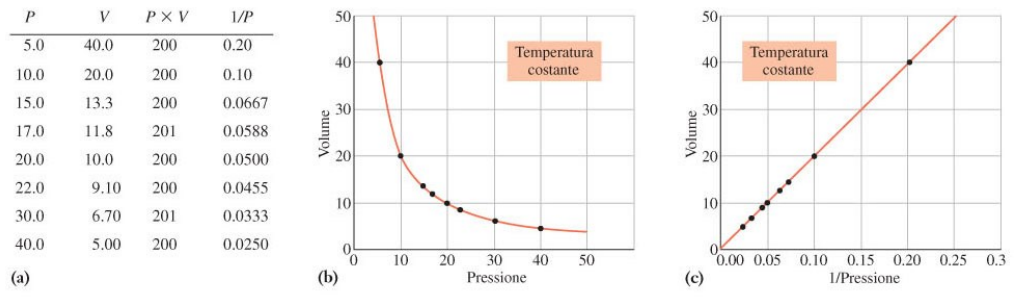
\includegraphics[width=15cm]{immagini/Legge_di_Boyle.png}
\end{figure}

La legge può essere espressa come $\displaystyle PV=k \qquad P=\frac{k}{V} \qquad V=\frac{k}{P}$

\vspace{0.2cm}o, in forma logaritmica, come $logV = logk - log P$
\subsection{Legge di Charles (Gay-Lussac)}
Se manteniamo costante la pressione (trasformazione isobara), il volume di un gas aumenterà rispetto a quello iniziale di un 273-esimo per ogni grado di aumento di temperatura:
$$p=cost \implies V_t=V_0(1 + \alpha t), \; \text{con} \; \alpha=\frac{1}{273}$$
$$\implies V_t=V_0 \left( \frac{273 + t}{273} \right), \; T=273 + t$$
$$\implies V_T = \frac{V_0 T}{273}, \; \frac{V_T}{T}=\frac{V_0}{273}=cost$$

E se la temperatura $T$ fosse pari a zero? Sarà zero anche il volume? No, in quanto nella pratica si ha la liquefazione del gas, cioè il volume diminuisce drasticamente perché si ha il liquido.

\vspace{0.2cm}Consideriamo ora un becher con acqua e ghiaccio (immaginiamo di essere a 0° C) nel quale è messa una provetta che al suo interno ha aria. Introfuciamo nella provetta alcune goccioline di mercurio (usiamo il mercurio perché può salire e scendere facilmente dato che è un liquido) in modo tale da formare un tappo di mercurio che comprime l'aria fino ad un certo punto per poi quindi bloccarsi.

\begin{figure}[htp]
    \centering
    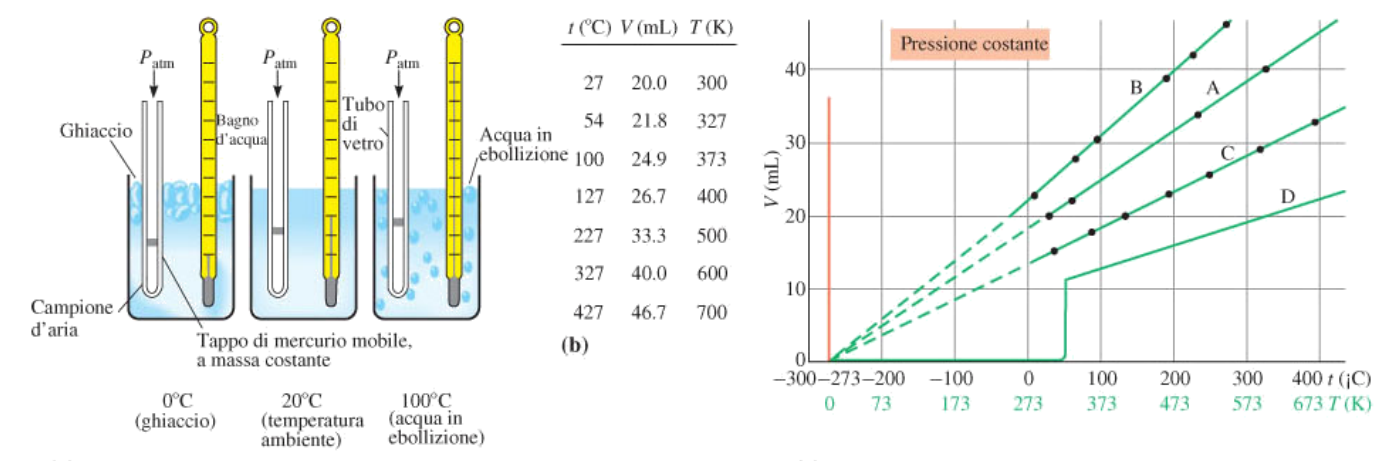
\includegraphics[width=15cm]{immagini/esperimento_provetta.png}
\end{figure}

Se riscaldiamo il sistema ci accorgiamo che il tappo di mercurio si alza, quindi sta cambiando pressione e volume. Se invece oltre a riscaldare manteniamo costante la pressione, noteremo che il volume cresce linearmente con la temperatura. Gli andamenti A, B e C sono quelli dei gas ideali fissati diversi valore di pressione, mentre l'andamento D è quello di un gas reale. In esso notiamo che, andando da destra verso sinistra, a un certo punto il volume crolla. Ciò significa che il gas si è liquefatto, ossia il volume crolla perché il gas si liquefa. Questa è la prova sperimentale che il volume non va a zero.
\subsection{Legge di Gay-Lussac}
Se manteniamo costante il volume (trasformazione isocora) la pressione del gas è proporzionale alla temperatura: per ogni grado di aumento di temperatura la pressione aumenta di 1/273-esimo del suo valore iniziale:

$$V=cost \implies p_t=p_0(1 + \alpha t), \; \text{con} \; \alpha=\frac{1}{273}$$
$$\implies p_t=p_0 \left( \frac{273 + t}{273} \right), \; T=273 + t$$
$$\implies p_T = \frac{p_0 T}{273}, \; \frac{p_T}{T}=\frac{p_0}{273}=cost$$

\subsection{Legge di Dalton e delle pressioni parziali}
Supponiamo di avere più di un gas ideale nel volume a disposizione. Abbiamo detto che un gas ideale è caraterizzato dall'assenza di interazione fra le particelle, per cui se tutti i gas presenti hanno tale comportamento non ci saranno interazioni fra le varie particelle, ossia ogni gas si comporta come se fosse l'unico presente nell'intero contenitore. Pertanto la pressione totale sarà pari alla pressione dei singoli gas:
$$P_{tot}=P_1 + P_2 + P_3 + ... + P_N = \sum_{i=1}^nP_i$$

Vediamo un esempio numerico:

\vspace{-0.3cm}
\hspace{0.5cm}\begin{minipage}{0.55 \textwidth}
    \begin{figure}[H]
        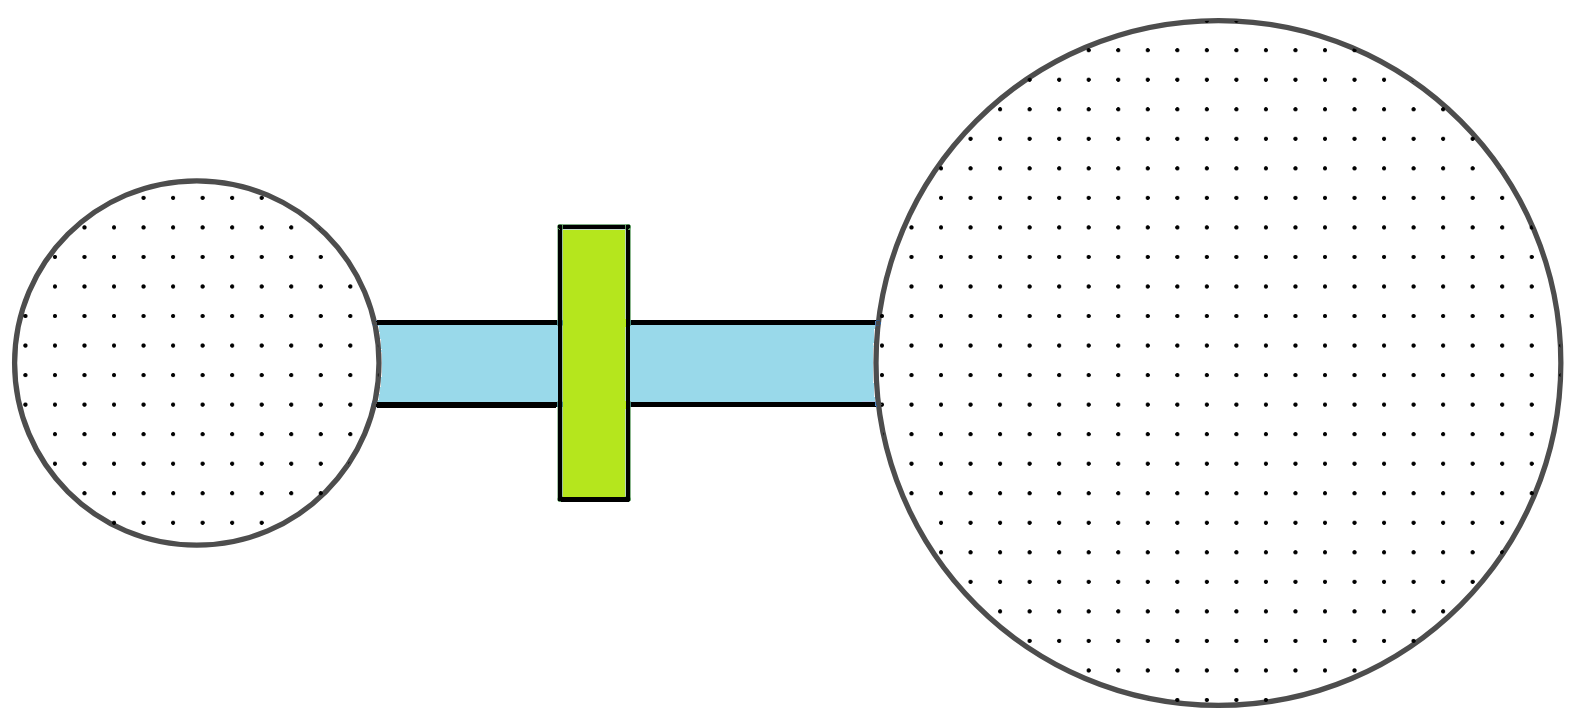
\includegraphics[width=8cm]{immagini/serbatoio.png}
    \end{figure}
\end{minipage}
\begin{minipage}{0.4 \textwidth}
\vspace{0.8cm}Consideriamo due recipienti che hanno al loro interno due gas diversi. Essi inoltre sono collegati con un rubinetto inizialmente chiuso.

Le condizioni iniziali sono

\begin{center}
    \begin{tabular}{p{2.5cm}p{2.5cm}}
        $p_1=175 \; torr$ & $p_2=125 \; torr$\\[1ex]
        $V_1=0.527 \; L$ & $V_2=3.141 \; L$
    \end{tabular}
\end{center}
\end{minipage}

\vspace{0.4cm}A temperatura costante vale $pV=cost$.

Il volume finale vale $V_{tot}=V_1 + V_2 =3.668 \; L$

Le pressioni parziali valgono

\vspace{0.2cm}$p_1V_1=p_x \cdot 3.668 \rightarrow 175 \cdot 0.527 = p_x \cdot 3.668 \rightarrow p_x = 25.14 \; torr$

\vspace{0.2cm}$p_2V_2=p_y \cdot 3.668 \rightarrow 125 \cdot 3.141 = p_y \cdot 3.668 \rightarrow p_y = 107.4 \; torr$

\vspace{0.2cm}La pressione totale vale $p_{tot}=p_x + p_y=25.14 + 107.04=132.18 \; torr$. Essa sarà la pressione esercitata dal volume $V_{tot}$, che è calcolata in funzione delle pressioni parziali grazie alla legge di Dalton.
\subsection{Legge dei volumi molare e di Avogadro}
Consideriamo le equazioni
$$\ce{H_2 + O_2 -> 2H_2O}$$
$$\ce{2CO + O_2 -> 2CO_2}$$
$$\ce{H_2 + Cl_2 -> 2HCl}$$
Esse sono tutte speci gassose.

Sperimentalmente si è visto che, se i gas vengono prelevati nelle stesse condizioni di temperatura e pressione i rapporti stechiometrici si mantengono anche se anziché considerare moli consideriamo volumi. Dunque, nei nostri esempi, 2 litri di H$_2$ più 2 litri di O$_2$ daranno luogo a 2 litri di H$_2$O in fase gassosa.

Quindi questi rapporti in moli sono rapporti anche in volumi. Da ciò segue la legge di Avogadro:
"\textit{Volumi uguali di gas diversi, nelle stesse condizioni di temperatura e pressione, devono contenere lo stesso numero di molecole. In particolare a 0° C e 1 atm una mole di qualunque gas occupa sempre un volume di} $22.414$ \textit{litri, che è detto volume molare}".

\vspace{0.2cm}Si definiscono \textbf{condizioni normali} 0° C e 1 atm.

\vspace{0.2cm}Si definiscono \textbf{condizioni standard} 25° C e 1 atm.

\vspace{0.2cm}Attenzione! In alcuni testi vengono etichettate, rispettivamente, come \textit{condizioni standard} e \textit{condizioni standard ambientali}. Useremo la prima nomenclatura.
Va da ricordare che una mole contiene $6.023 \cdot 10^23$ particelle, tale numero si può determinare così:

Consideriamo il radio. Esso dà luogo per disintegrazione al radon più particelle $\alpha$, le quali sono atomi di elio doppiamente ionizzati:

$$\ce{^{226}_{88}Ra -> ^{222}_{86}Rn + \alpha \; \text{+ energia,} \qquad \alpha= ^{4}_{2}He^{2+}}$$
\subsection{Equazione di stato}
\subsection{Determinazione dei pesi molecolari}
\subsection{Gas e vapori}